\documentclass[10.5pt]{article} 
\usepackage[intlimits]{amsmath} % AMS Math Package
\usepackage{amsthm} % Theorem Formatting
\usepackage{amssymb} % Math symbols such as \mathbb
\usepackage{graphicx} % Allows for eps images
\usepackage{multicol} % Allows for multiple columns
\usepackage[dvips,letterpaper,margin=1in,bottom=1in]{geometry}
\usepackage{multirow}
\usepackage{booktabs}
\usepackage{bigstrut}
\usepackage[table]{xcolor}
\usepackage[hidelinks]{hyperref}
\usepackage{mathrsfs}
\usepackage{amsmath,amscd}
\usepackage[all,cmtip]{xy}
\usepackage{bbm}
\usepackage[centercolon]{mathtools}
\usepackage{fontspec}

\usepackage{ctex}

\usepackage{abstract}

\usepackage{lipsum}
\usepackage{tikz}
\usepackage{tikz-cd}

\usepackage{geometry}
\geometry{papersize={210mm,297mm}}
\geometry{left=2cm,right=2cm,bottom=1.5cm}

\usepackage{indentfirst}
\setlength{\parindent}{2em}

\usepackage[utf8]{inputenc}

\usepackage{abstract}
\usepackage{caption}
\usepackage{float}
\usepackage{mhchem}
%\usepackage{physics}
\usepackage{physunits}
\usepackage{bm}
\usepackage{ulem}
\usepackage{upgreek}

\usepackage{url}
\usepackage{tikz-3dplot}

\usepackage[siunitx]{circuitikz}
\usepackage{subfig}

\usetikzlibrary{decorations.pathreplacing}

%\usepackage{ntheorem}
%空白页
\usepackage{afterpage}
\newcommand\myemptypage{
	\null
	\thispagestyle{empty}
	\addtocounter{page}{-1}
	\newpage
}




%方括号文献
%\usepackage[square]{natbib}


%自定义颜色
% 定义一个较暗的橘黄色
\definecolor{darkorange}{rgb}{0.8, 0.4, 0.0}

%以下是自定义命令区
\newcommand\rme{\mathrm{e}}
\newcommand\rmi{\mathrm{i}}
\newcommand\rmmax{\mathrm{max}}
\newcommand\rmmin{\mathrm{min}}
\newcommand\G{\text{Galois}}
\newcommand\rmG{\mathrm{Galois}}
\newcommand\Aut{\mathrm{Aut}}
\newcommand\Gal{\mathrm{Gal}}
\newcommand{\cate}[1]{\ensuremath{\mathsf{#1}}}	% Font series for categories



\newcommand*{\titleGM}{
	\begingroup % Create the command for including the title page in the document
	\hbox{ % Horizontal box
		\hspace*{0.2\textwidth} % Whitespace to the left of the title page
		\rule{1pt}{\textheight} % Vertical line
		\hspace*{0.05\textwidth} % Whitespace between the vertical line and title page text
		\parbox[b]{0.75\textwidth}{ % Paragraph box which restricts text to less than the width of the page
			
			{\noindent\Huge\bfseries 近代物理实验II \\}\\[2\baselineskip] % Title
			{\large \textit{X射线的产生与X射线谱}}\\[4\baselineskip] % Tagline or further description
			{\large \textsc{Xichen Li}} 
			\\[1\baselineskip]% Author name
			{\begin{figure}[H] % 创建一个 figure 环境
				\includegraphics[scale=0.35]{cover.jpg}
			\end{figure}}%cover figure
			%可加入封面图
			\vspace{0.2\textheight} % Whitespace between the title block and the publisher
			%{\noindent 李熙宸}\\[\baselineskip]
			{\noindent Email:xichen.li@bnu.edu.cn}\\[\baselineskip] % Publisher and logo
	}}\endgroup}

% Sets margins and page size
\pagenumbering{arabic}
\pagestyle{headings} % Removes page numbers
\makeatletter % Need for anything that contains an @ command 
\renewcommand{\maketitle} % Redefine maketitle to conserve space
{ \begingroup \vskip 10pt \begin{center} \Huge {\bf \@title}
		\vskip 10pt \large \@author \hskip 20pt \@date \end{center}
	\vskip 10pt \endgroup \setcounter{footnote}{0} }
\makeatother % End of region containing @ commands
\renewcommand{\labelenumi}{(\alph{enumi})} % Use letters for enumerate
% \DeclareMathOperator{\Sample}{Sample}
\let\vaccent=\v % rename builtin command \v{} to \vaccent{}
\renewcommand{\v}[1]{\ensuremath{\mathbf{#1}}} % for vectors
\newcommand{\gv}[1]{\ensuremath{\mbox{\boldmath$ #1 $}}} 
% for vectors of Greek letters
\newcommand{\uv}[1]{\ensuremath{\mathbf{\hat{#1}}}} % for unit vector
\newcommand{\abs}[1]{\left| #1 \right|} % for absolute value
\newcommand{\avg}[1]{\left< #1 \right>} % for average
\let\underdot=\d % rename builtin command \d{} to \underdot{}
\renewcommand{\d}[2]{\frac{\mathrm{d} #1}{\mathrm{d} #2}} % for derivatives
\newcommand{\dd}[2]{\frac{\mathrm{d}^2 #1}{\mathrm{d} #2^2}} % for double derivatives
\newcommand{\pd}[2]{\frac{\partial #1}{\partial #2}} 
% for partial derivatives
\newcommand{\pdd}[2]{\frac{\partial^2 #1}{\partial #2^2}} 
% for double partial derivatives
\let\baraccent=\= % rename builtin command \= to \baraccent
\renewcommand{\=}[1]{\stackrel{#1}{=}} % for putting numbers above =
\providecommand{\wave}[1]{\v{\tilde{#1}}}
\providecommand{\fr}{\frac}
\providecommand{\RR}{\mathbb{R}}
\providecommand{\CC}{\mathbb{C}}
\providecommand{\NN}{\mathbb{N}}
\providecommand{\e}{\epsilon}
\newcount\colveccount
\newcommand*\colvec[1]{
	\global\colveccount#1
	\begin{pmatrix}
		\colvecnext
	}
	\def\colvecnext#1{
		#1
		\global\advance\colveccount-1
		\ifnum\colveccount>0
		\\
		\expandafter\colvecnext
		\else
	\end{pmatrix}
	\fi
}

\title{\huge{X射线的产生与X射线谱}}
\author{\small{李熙宸202111140061}}
\date{2024/03/29}

%汉化相关内容
\renewcommand{\contentsname}{\centering 目录}
\renewcommand{\abstractname}{\textbf{摘\quad 要}} %更改摘要二字的样式
\renewcommand{\refname}{参考文献}

%两级目录
\setcounter {tocdepth} {2} 

%此后尝试修改字体
\newtheorem{thm}{定理}[section]
\newtheorem{lem}[thm]{引理}
\newtheorem{prop}[thm]{命题}
\newtheorem{corollary}[thm]{推论}
\theoremstyle{definition}
\newtheorem{dfn}{定义}[section]
\newtheorem{example}{例}[section]
\theoremstyle{remark}
\newtheorem{rmk}{注}[section]
\newenvironment{solution}{\begin{proof}[\bf 解]}{\end{proof}}
\renewcommand{\proofname}{\bf 证明}

%\newtheorem{thm}{定理}[section]
%\newtheorem{prop}{命题}[thm]
%\newtheorem{problem}{Problem}[thm]
%\usepackage{cancel}
%\newtheorem{lem}{引理}[thm]
%\theoremstyle{definition}
%\newtheorem{dfn}{定义}[thm]
%\theoremstyle{remark}
%\newtheorem{rmk}{Remark}  [thm]
%\newenvironment{solution}{%\small%
	%	\begin{trivlist} \item \textit{Solution}.  }{%
		%		\hspace*{\fill} $\blacksquare$\end{trivlist}}
%\pagestyle{myheadings}

% ***********************************************************
% ********************** END HEADER *************************
% ***********************************************************

\begin{document}
	%去除封面编号
	\pagestyle{empty}
	\titleGM
	\myemptypage
	\tableofcontents
	\newpage
	\myemptypage
	\pagestyle{headings}
	\setcounter{page}{1}
	\maketitle
	\begin{abstract}
		本实验简要介绍了X射线的产生原理,探讨了X射线谱的规律、X射线与物质的相互作用以及X射线光谱分析方法。研究了单晶的布拉格衍射现象,发现钼靶材料对应的X射线标识谱中有两条特征峰值波长,分别为$\lambda_1=0.061$ nm和$\lambda_2=0.069$ nm。还研究了X射线管的电压及其对X射线谱的影响,验证了Duane-Hunt关系,并计算出普朗克常量为$h=6.7119\times10^{-34};\text{J}\cdot\text{s}$,相对误差为1.29%。
	
	\end{abstract}
	\section{引言}
	1895年德国物理学家伦琴在研究阴极射线时发现了X射线,其在医疗上和金属探伤上有重大的应用价值,为多种科学领域提供了一种有效的研究手段。
	
	
	在科学家探索X射线本质的过程中,1912年劳厄等人发现了X射线在晶体上的衍射现象,证实X射线是波长在0.1nm左右的电磁波;在研究X射线性质时,巴克拉发现X射线具有标识谱,即从各种元素发出的标识X射线带有原子内部结构的信息,这对建立原子结构理论极为重要,随后莫塞莱在巴克拉的基础上发现元素发出的标识X射线能量与原子序数之间的关系,即莫塞莱定律。 
	
	
	为了了解X射线谱的规律,X射线和物质的相互作用及X射线光谱分析方法,我们在本实验中用能谱色散的方法分析X射线标识谱,验证莫塞莱定律,并测定X射线通过物质的指数衰减规律以及吸收常数在某些能量处所发生的突变。\cite{X射线的产生与X射线谱}
	\section{原理}
	\subsection{X 射线的产生及 X 射线谱}
	实验室中产生X射线最常用的方法是利用X射线管,现在常用的X射线管多属于高真空热阴极。X 射线管要产生 X 射线必须具备下列条件:第一,能产生足够数量电子的阴极和能经受高速电子撞击而产生X 射线的阳极靶面;第二,高真空管,以使得电子不受阻碍而降低能量,同时保护灯丝不致氧化而烧毁;第三,管两端以阳极为正极,阴极为负极的高电压。X射线管中高速电子撞击阳极靶面时,仅不到1\%的能量转变为X射线,绝大部分能量转换为热能,故X 射线管工作时,阳极靶面要水冷或风冷,避免温度急剧升高。
	
	X射线谱指的是X射线的强度随波长变化的关系曲线。X射线管发出的典型的X射线 谱可分为两个部分:一部分是连续谱,谱线连续平滑分布,用不同动能的电子轰击靶材时,产生的连续谱形状相似,而且都有最短波长$\lambda_{\min},\lambda_{\min}$与管电压V有关;另一部份是线状谱,谱线是几个尖锐的、分立的峰,其峰值波长与 X 射线管工作条件无关,只取决于靶材的化学元素,也被称为标识谱。
	
	连续谱由轫致辐射产生。高速电子打到阳极靶上,在与靶原子碰撞过程中损失的能量的一部分或全部转化为辐射能,产生的辐射被称为轫致辐射。绝大多数电子要和靶物质进行多次碰撞,逐次丧失能量,直至完全耗尽为止。故轫致辐射产生的X 射线谱是连续谱。此连续谱的短波极限$\lambda_{\min}$对应着入射电子一次碰撞就失去全部动能的情况,而X射线管中电子动能通过X射线管管电压V加速获得,可知有
	\begin{equation}\label{eq:DH}
		\lambda_{\min}=\dfrac{hc}{eV}=\dfrac{1.24\times10^3}{V}\nm
	\end{equation}
	其中$U$的单位为Volt(V), 此式被称为Duane-Hunt关系,若实验中测出 $U$ 和$\lambda_{\min},$也可由该式算出Planck常量$h$。
	
	轫致辐射的强度与阳极靶的原子序素Z 有关,频率分布由入射的高速电子能量决定。 
	实验发现,轫致辐射产生的连续谱的性质与X 射线管的管电压$U$、管电流$I$和靶材料这三个因素有关:
	\begin{itemize}
		\item 管电压$U$升高时,所有波长的X射线强度均增加,同时短波限$\lambda_{\min}$向短波方向移动,强度最高的X射线波长$\lambda_{\max}$也随之向短波方向移动;
		\item 管电压$U$不变,增大管电流$I$,各种波长X射线相对强度增加,但$\lambda_{\min}$和$\lambda_{\max}$不变
		\item 若保持管电压和电流一定,改变阳极靶材,随着阳极物质原子序数Z 的增加,各种波长的X 射线的相对强度增大,整个曲线向上方移动,但$\lambda_{\min}$和$\lambda_{\max}$均不变;
		\item 对连续谱进行积分可得到连续谱的强度$I_{\text{连}}$,其满足$I_{\text{连}}$=$k_{\text{连}} IZV^2$
	\end{itemize}
	
	标识X 射线是在连续X 射线的基础上产生的,当管电压V提高到某一临界值后,便会在连续谱上一定波长处出现离散的、强度很高的线状谱,线状谱的强度受管电压影响,峰位与管电压无关,只由阳极靶的材料决定。
	
	标识谱的产生机理与阳极物质的原子结构相关。当靶面被高速粒子轰击时,可能出现处于高能级的激发态,激发态不稳定,以光量子的形式释放出能量,其频率满足:$h\nu=E_{n_2}-E_{n_1}$。激发态原子的不同外层电子 向 K层跃迁时产生的辐射统称为 K系辐射,其中,电子由L层跃迁到K层所产生的X射线称$\mathbb{K}_\alpha$射线,考虑到由于同一能级层的精细结构,跃迁产生的谱线也有相应的精细结构,按波长减小依次用数字1、2 等标记。
	
	系列实验证明, X 射线标识谱的分布有如下实验规律:
	\begin{itemize}
		\item X 射线标识谱峰位由其原子的能级结构决定,对于一定的阳极靶材料,其特征波长有确定值,与管电压和管电流等实验条件无关,也与元素的化合状态无关;
		\item 只有当管电压高于临界值$V_{\text{th}}$时,连续谱才会伴有标识谱,称$V_{\text{th}}$为X 射线标识谱的激发电压。对不同的阳极靶材料,激发电压不同,其大小由阳极靶的原子序数Z 决定。对于钼靶X 光管,只有电压高于20 kV 时,才会产生标识谱
		\item 当管电压$U$超过激发电压$V_{\text{th}}$且升高时,X 射线标识谱的强度随管电压$U$、管电流$I$和激发电压$V_{\text{th}}$的变化规律满足
		\begin{equation}
			I_{\text{标识}}=k_{\text{标识}}I(V-V_{\text{th}})^m
		\end{equation}
		对于K线系$m=1.5,$L系 $m=2$。
	\end{itemize}
	\subsection{X 射线与物质的相互作用}
	X 射线与物质的相互作用有
	\begin{itemize}
		\item 光电效应\\
		在光子-电子的相互作用中,如果光子的能量≥核对电子的束缚能,电子就可能吸收光子的全部能量而被电离成为自由电子。
		\item 康普顿散射\\
		当X 射线与原子中的价电子或自由电子相互作用时,由于能动量守恒,散射过后出射光子波长改变量满足
		\begin{equation}
			\Delta\lambda=\dfrac{h}{m_ec}(1-\cos2\theta)
		\end{equation}
		\item 相干散射\\
		入射 X 射线与原子中束缚较强的电子相互作用时,在入射X射线交变电场的作用下,电子将被迫围绕其平衡位置发生振动,振动频率与入射X 射线的频率相同,并向四周发射与其振动频率相同的电磁波,这种散射X 射线的波长、频率均与入射线相同,在相同的传播方向上可以发生干涉现象,故称为相干散射。
		
		当X 射线在晶体中各原子的电子上发生散射时,由于晶体中原子排列是有规律、周期性的,且原子间距与X 射线波长数量级相近,散射波中与原射线波长相同的相干散射波将互相干涉,在特定方向上产生衍射线。晶体衍射方向决定于晶体微观结构的类型及其基本尺寸(晶面间距,晶胞参数等);衍射线的强度决定于晶胞中各组成原子的元素种类及其分布排列的坐标。
		\begin{figure}[H]
			\centering
			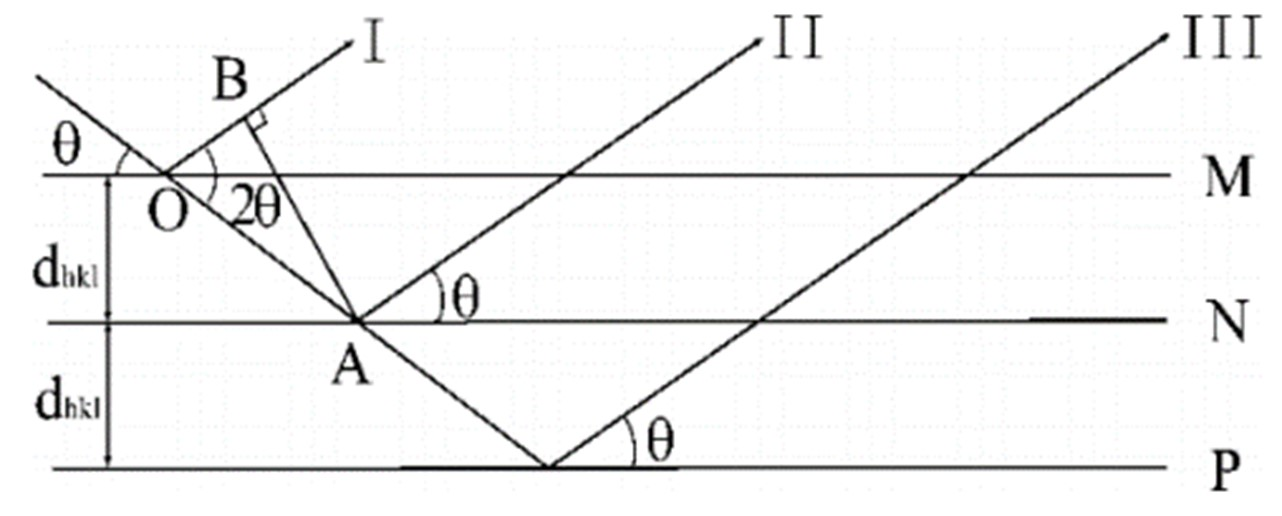
\includegraphics[scale=0.4]{1.jpg}
			\captionsetup{font=footnotesize}
			\caption{X 射线在晶面族上的衍射}
		\end{figure}
		如Figure 1,晶体相邻晶面上反射的X射线光程差为$\delta=2d\sin\theta$,当$\delta$为入射X射线波长$\lambda$的整数$n$倍时
		\begin{equation}\label{eq:blg}
			2d\sin\theta=n\lambda,\quad n\in\mathbb{Z}
		\end{equation}
		将产生第$n$级干涉极大,式(\ref{eq:blg})称为布拉格方程。
	\end{itemize}
	\subsection{X射线衍射仪}
	X射线衍射仪通常由X射线发生器、测角仪及控制系统、X 射线探测器及相应的数据采集和处理分析软件构成, 结构示意图如Figure 2所示。X 射线管发出的X 射线经光阑准直后照射到待测样品上,衍射线经探测器采集。样品台和探测器支架分别装在测角仪的两个同轴转盘上,以$\theta:2\theta$的方式连动,以记录不同方向上的衍射线强度。测角仪是衍射仪中最精密的机械部分,是衍射仪的核心部分。
	\begin{figure}[H]
		\centering
		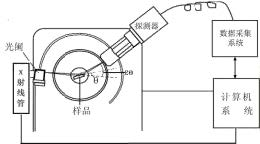
\includegraphics[scale=0.7]{2.jpg}
		\captionsetup{font=footnotesize}
		\caption{X 射线衍射仪结构示意图}
	\end{figure}
	\section{实验步骤}
	\begin{itemize}
		\item [1.] 单晶的布拉格衍射研究\par 
		检查仪器无误后,安装氯化钠单晶样品:带手套操作,仅接触样品短边;固定时轻轻卡住。
		
		设置X 射线管工作条件:高压$U=35$ kV,电流$I=1.00$ mA,按(COUPLED)按钮,选择样品臂与探测臂耦合扫描方式,设置$\beta_{\min}=2^\circ,\beta_{\max}=25^\circ$,步幅$\Delta\beta=0.1^\circ$,各角度测量时长$\Delta t=10 $s,然后在按仪器控制区下方“SCAN”按钮等待扫描
		\item [2.] 研究X射线管的电压对于X射线谱的影响\par 
		设置$U=15$ kV,$I=1$ mA,$\beta_{\min}=2^\circ,\beta_{\max}=10^\circ$,其余设置不变然后扫描。
		
		隔5 kV改变一次电压,直至35 kV,其余设置不变并扫描,保存数据和曲线并分析。
		
		\item [3.]研究X射线管的电流对于X射线谱的影响\\
		设置$U=35$ kV, $I=0.4$ mA,$\beta_{\min}=6^\circ,\beta_{\max}=7.5^\circ$。隔$0.1$ mA改变一次电流,直至$1$ mA,其余设置不变并扫描,保存数据和曲线并分析。
	\end{itemize}
	\section{结果与分析讨论}
	\subsection{单晶布拉格衍射}
	根据Figure 3可以看到$\beta:2^\circ\sim25^\circ$范围内一共有六个衍射峰,对应三个衍射级次,选取$U=35 $kV的谱线并结合式(\ref{eq:blg})计算得衍射波长如下表($d=0.282 $nm)
	% Table generated by Excel2LaTeX from sheet 'Sheet3'
	\begin{table}[htbp]
		\centering
		\caption{X射线谱特征波长计算,$U=35 $kV}
		\begin{tabular}{|c|c|c|c|c|c|c|}
			\hline
			$n$     & \multicolumn{2}{c|}{1} & \multicolumn{2}{c|}{2} & \multicolumn{2}{c|}{3} \bigstrut\\
			\hline
			$\theta/^\circ$ & 6     & 6.9   & 12.6  & 14.2  & 19.3  & 21.9 \bigstrut\\
			\hline
			$\lambda_1/$nm & 0.059  &       & 0.062  &       & 0.062  &  \bigstrut\\
			\hline
			$\lambda_2/$nm &       & 0.068  &       & 0.069  &       & 0.070  \bigstrut\\
			\hline
			$\overline{\lambda}_1/$nm& \multicolumn{6}{c|}{0.061 } \bigstrut\\
			\hline
			$\overline{\lambda}_2/$nm& \multicolumn{6}{c|}{0.069 } \bigstrut\\
			\hline
		\end{tabular}%
	\end{table}%
	
	该阳极材料对应的X射线标识谱只有两条峰值波长,分别为
	\begin{align}
		\lambda_1&=0.061\nm\\
		\lambda_2&=0.069\nm
	\end{align}
	\begin{figure}[H]
		\centering
		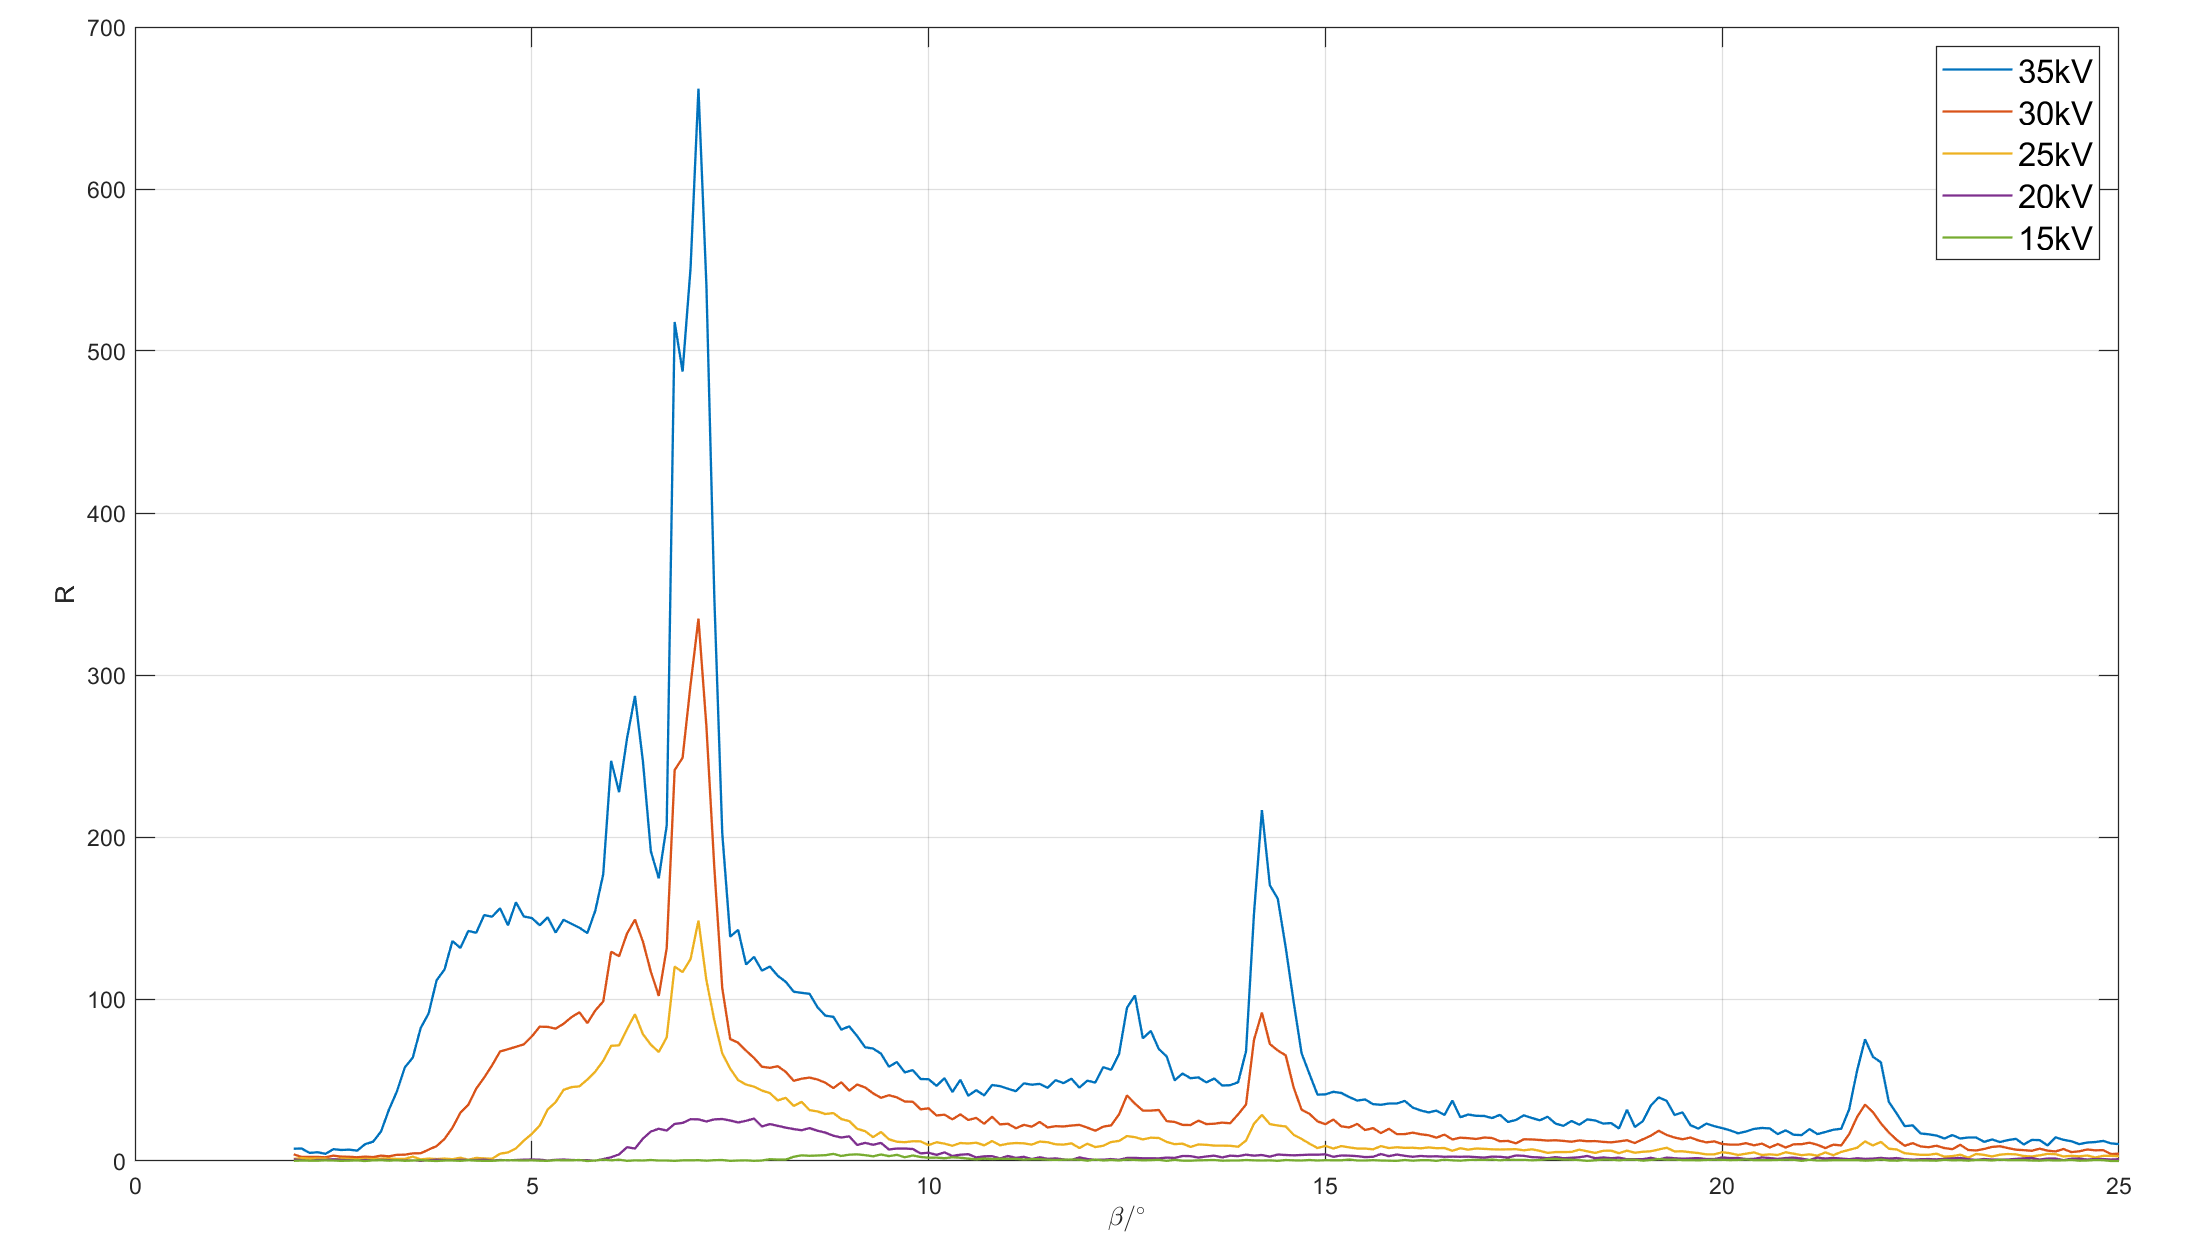
\includegraphics[scale=0.65]{voltage.png}
		\captionsetup{font=footnotesize}
		\caption{从上到下电压为$35,30,25,20,15$ kV对应相对强度随样平台相对初始平行线转过角度$\beta$的变化情况}
	\end{figure}
	接着改变电压大小,并保持电流$I=1$ mA不变,本次实验测量了电压$15\sim35$ kV范围五条衍射谱线,通过分析我们得到以下结论
	\begin{itemize}
		\item 针对连续谱,从Figure 3可以看到,随着管电压$U$升高时,所有波长的X射线强度均增加,同时短波限$\lambda_{\min}$向短波方向移动;
		\item 针对标识谱,我们可以看到改变电压,峰值波长对应的样平台转过角度不变,即峰值波长不变,即X 射线标识谱峰位与管电压无关;
		\item Figure 3中只有最上面的三条谱线同时有连续谱和标识谱,而$U=15$ kV,$20$ kV对应的X 射线只有连续谱,这说明只有当管电压高于临界值$V_{\text{th}}$时,连续谱才会伴有标识谱,且连续谱对应的电压应该处于$20\sim25$ kV范围内,具体研究见后。
	\end{itemize}
	
	实验第一次尝试测量时,峰值波长强度极小,而在调整了样平台与探测器之间的距离,以及重新放样品等操作后,峰值波长强度增大了10倍,但与Figure 3的最大值仍然有10倍的差距,这主要来源于测试角度问题,探测器与样平台相对初始平行线之间的角度不严格呈$2:1$的关系,大部分对应角度的X射线并未被探测器检测到,而在软件校准之后,角度校准,相应角度的X射线基本被检测到,所测强度也接近真实该角度的X射线强度。
	
	总结误差分析如下:
	\begin{itemize}
		\item 角度测量精度不够,步幅$\Delta\beta=0.1^\circ$,测量出的角度并非严格峰值,是主要的误差来源。
		\item 出射光为非平行光,出射口和探测口存在一定的宽度,带来测量上一定的误差,但不是主要因素。
	\end{itemize}
	\subsection{探究钼靶临界值$V_{\text{th}}$}
	根据Figure 4,我们可以看到当$U>20$ kV时,扫描出来的图像始终存在峰值,当$U=20$ kV时(对应倒数第二根曲线)曲线无峰值,得出$V_{\text{th}}=20$ kV,与理论值相符。
	
	仔细观察各条曲线,我们看到从(上往下)第五条曲线开始,曲线存在峰值,但峰值不在$\theta=7.2^\circ$,这说明实验存在较大的误差,由于存在噪声,再加上电压较小故扫描曲线的相对强度较小,因此噪声的存在影响判断曲线是否存在峰值。同时,误差也来源于样品移位,不断重复实验,改变样品角度的过程造成样品移位,故峰值不再准确。实验选取时间常数为$T=10$ s,可以考虑增大时间常数来降低噪声影响。
	\begin{figure}[H]
		\centering
		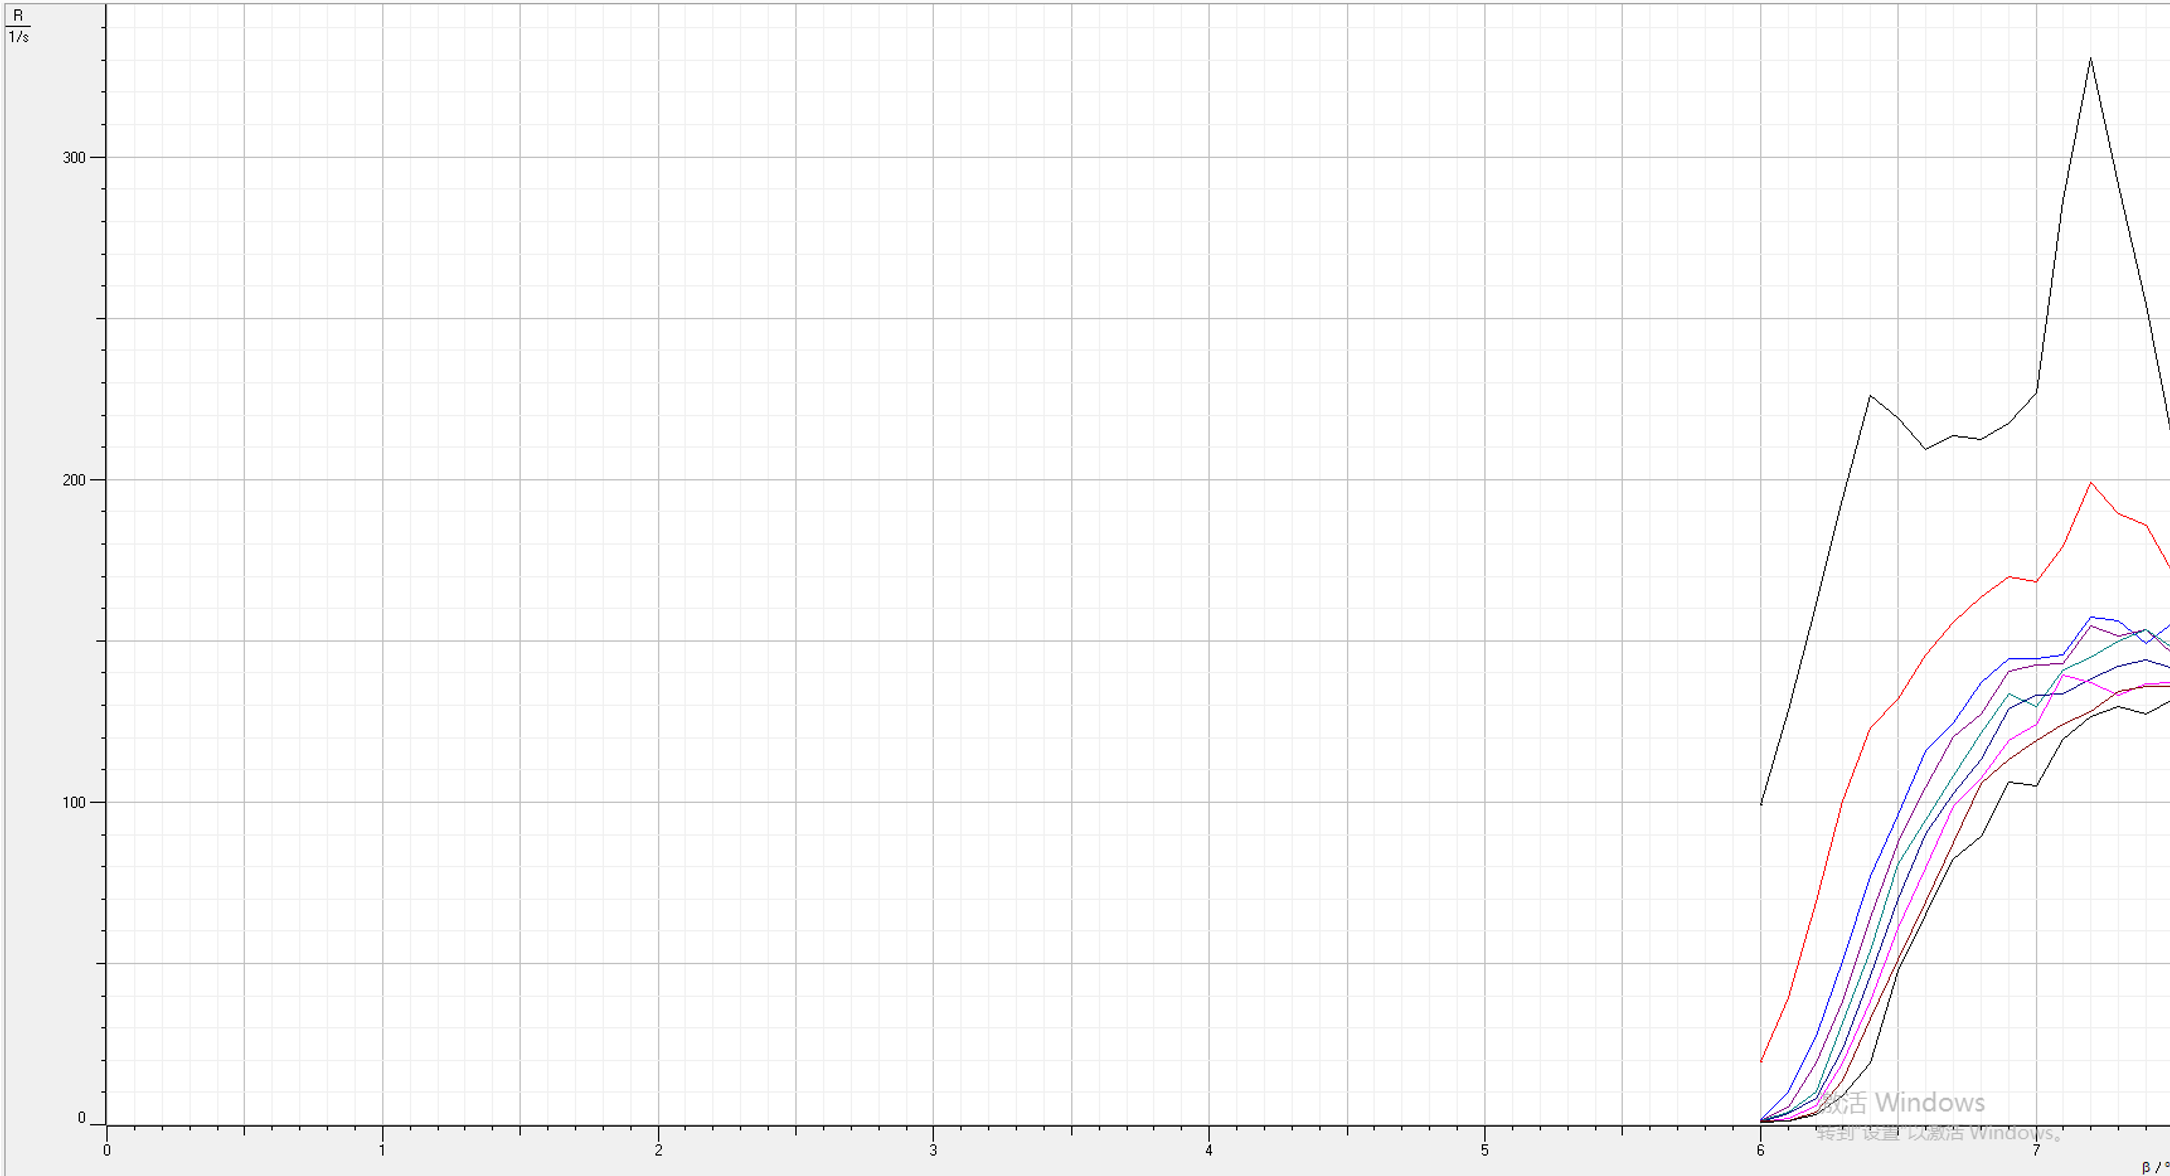
\includegraphics[scale=0.4]{vth.png}
		\captionsetup{font=footnotesize}
		\caption{从上到下电压为$22,21,20.5,20.4,20.3,20.2,20.1,20,19.9$ kV对应相对强度随样平台转过角度$\beta$的变化情况}
	\end{figure}
	\subsection{Duane-Hunt关系验证与普朗克常量计算}
	利用Duane-Hunt关系(\ref{eq:DH})和布拉格衍射方程(\ref{eq:blg})分别计算短波限$\lambda_{\min}$(电压$U:15\sim35$ kV),记作$\lambda_{\text{dh}},\lambda_{\text{brg}}$,所得结果如下表
	% Table generated by Excel2LaTeX from sheet 'Sheet3'
	\begin{table}[htbp]
		\centering
		\caption{利用Duane-Hunt关系和布拉格方程计算短波极限$\lambda_{\min}$}
		\begin{tabular}{|c|c|c|c|c|c|}
			\hline
			$U/$kV  & 15    & 20    & 25    & 30    & 35 \bigstrut\\
			\hline
			$\theta/^\circ$     & 8.4   & 6.1   & 4.7   & 3.7   & 2.8 \bigstrut\\
			\hline
			$\lambda_{\text{brg}}/$nm   & 0.082  & 0.060  & 0.046  & 0.036  & 0.028  \bigstrut\\
			\hline
			$\lambda_{\text{dh}}/$nm    & 0.083  & 0.062  & 0.050  & 0.041  & 0.035  \bigstrut\\
			\hline
		\end{tabular}%
	\end{table}%
	其中$U=15 $kV的峰值相对强度很低,误差可能较大。\\
	\begin{figure}[H]
		\centering
		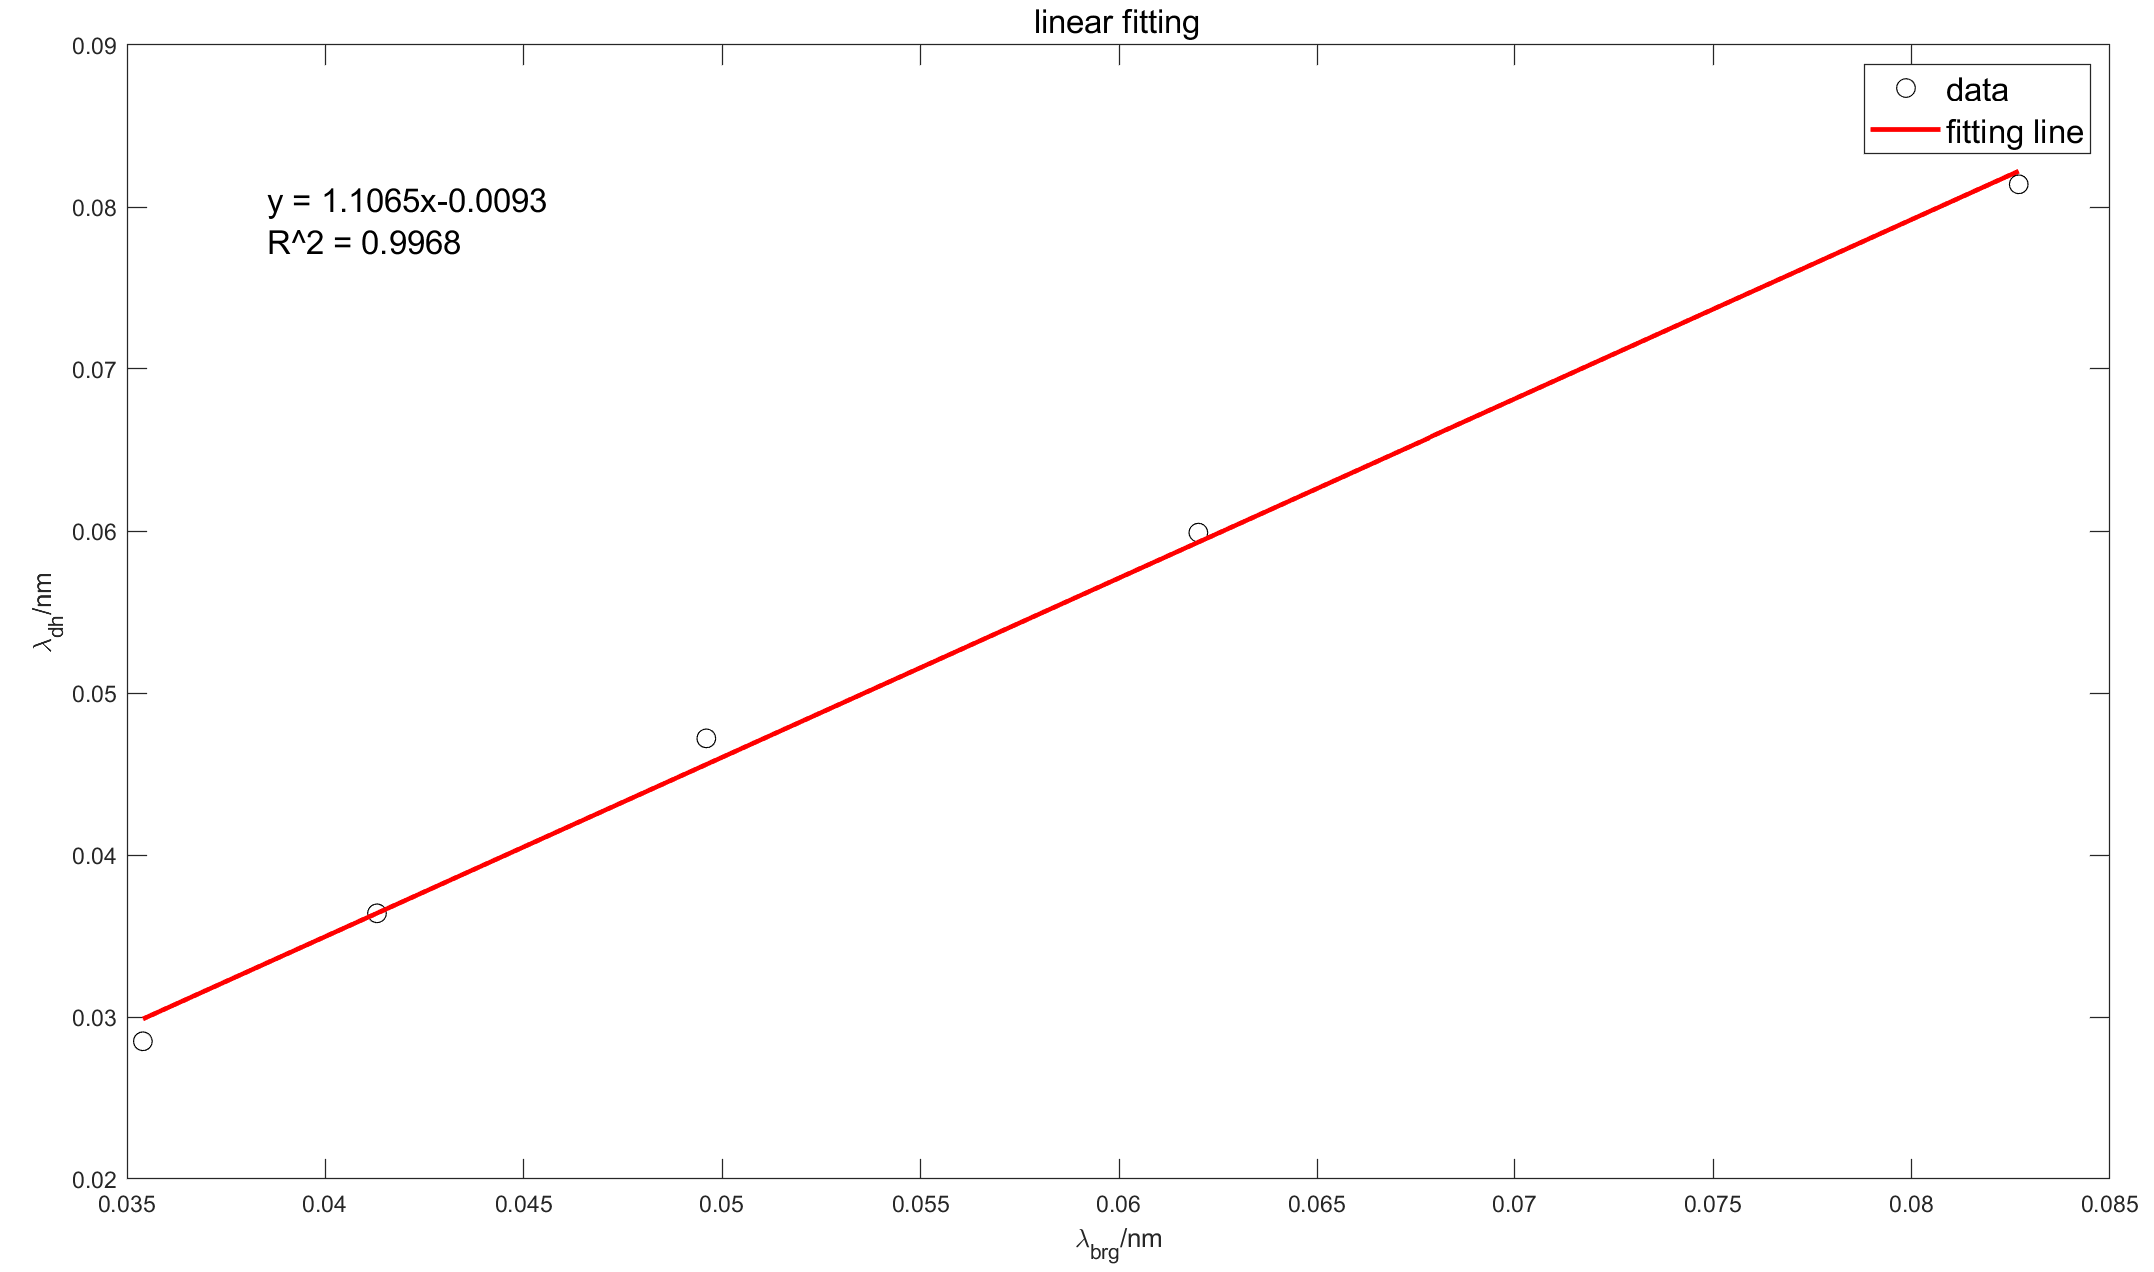
\includegraphics[scale=0.5]{dh_brg.png}
		\captionsetup{font=footnotesize}
		\caption{比较Duane-Hunt关系和布拉格方程计算的$\lambda_{\min}$}
	\end{figure}
	
	如Figure 5所示,采用Python scipy.stats模块的linregress工具作线性拟合得
	\begin{equation}\label{eq:fitting_dh}
		\lambda_{\text{dh}}=0.892\lambda_{\text{brg}}+0.009(\nm),\qquad R^2=0.9993901058
	\end{equation}
	
	这说明在实验误差允许范围内$\lambda_{\text{brg}}=\lambda_{\text{dh}}$,即理论值与实验值相等,也就验证了理论:Duane-Hunt关系的正确性。
	\begin{figure}[H]
		\centering
		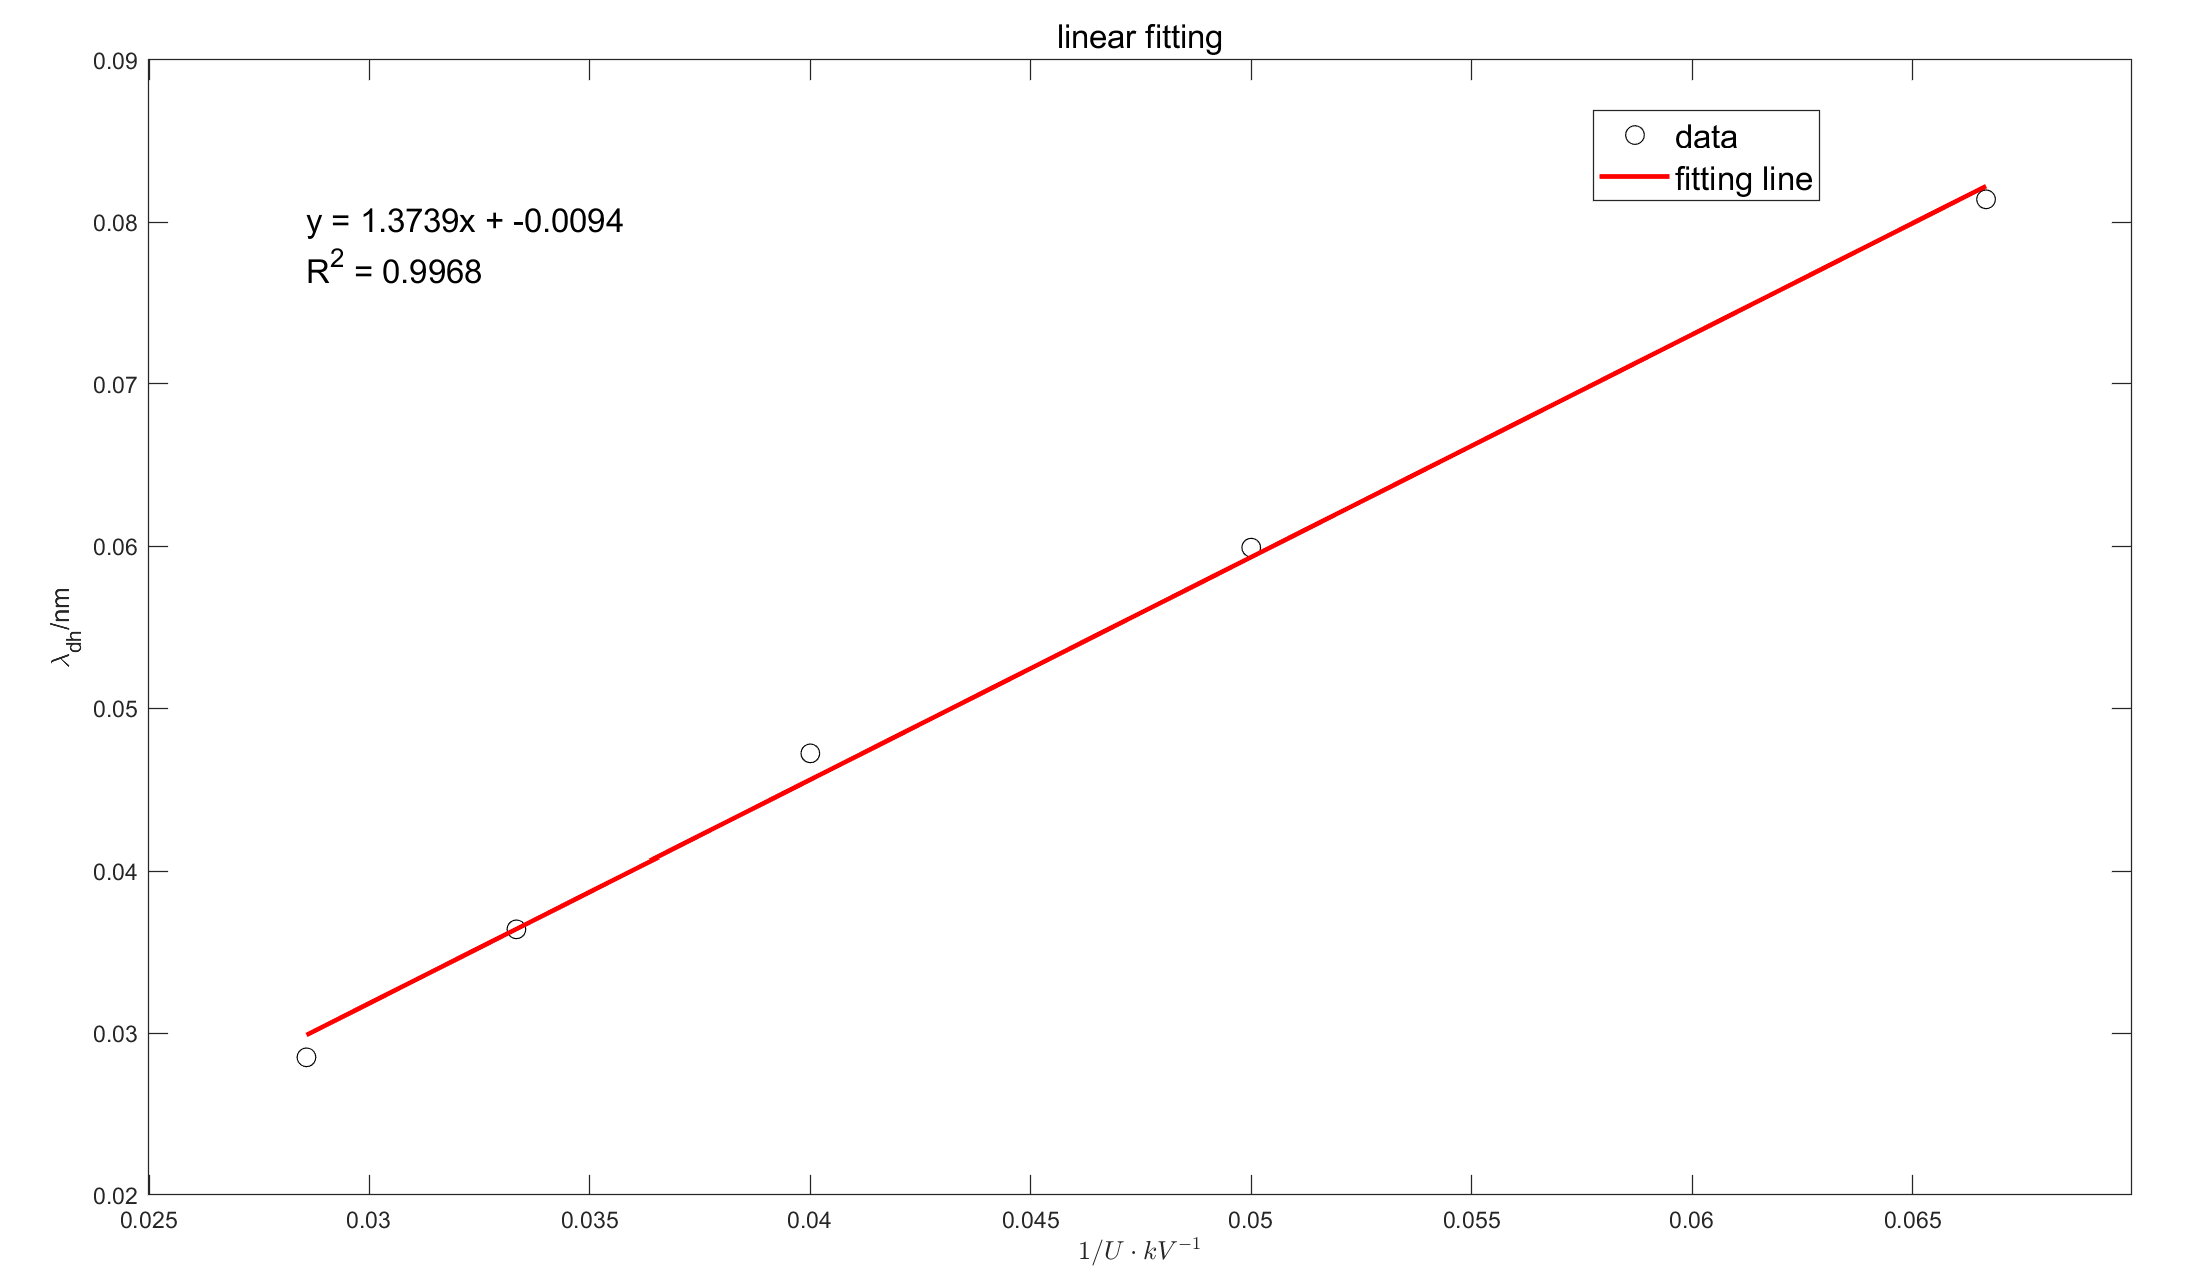
\includegraphics[scale=0.45]{lu.png}
		\captionsetup{font=footnotesize}
		\caption{短波极限$\lambda_{\min}$与X射线管管电压$U$倒数的关系}
	\end{figure}
	接下来,我们研究通过拟合方程(\ref{eq:fitting_dh})计算的短波限$\lambda_{\min}$与X射线管管电压$U$的倒数的关系,并作线性拟合,得到
	\begin{equation}
		\lambda_{\min}=\dfrac{1.2559\;\text{kV}}{U}-0.0007 (\nm),\qquad R^2=0.9991820854
	\end{equation}
	在误差允许范围内,$\lambda_{\min}$与$1/U$成正比,比例系数$k=1.2559\;\text{kV}\cdot\nm$, 带入光速$c$和电子电荷量$e$后,计算得出普朗克常量
	\begin{equation}
		h=\dfrac{ek}{c}=6.7119\times10^{-34}\;\text{J}\cdot\text{s}
	\end{equation}
	与实际值$h_{\text{re}}=6.62607015\times10^{-34}\;\text{J}\cdot\text{s}$的相对误差为$\delta=1.29\%$。
	
	\begin{itemize}
		\item 角度测量精度不够,步幅$\Delta\beta=0.1^\circ$,测量出的角度并非严格峰值,是主要的误差来源。
		\item 短波极限附近的相对强度极小,噪声的影响较大导致人工选择短波极限所对应的角度存在一定误差,是主要的误差来源。
	\end{itemize}
	\subsection{研究X射线管的电流对于X射线谱的影响}
	\begin{figure}[H]
		\centering
		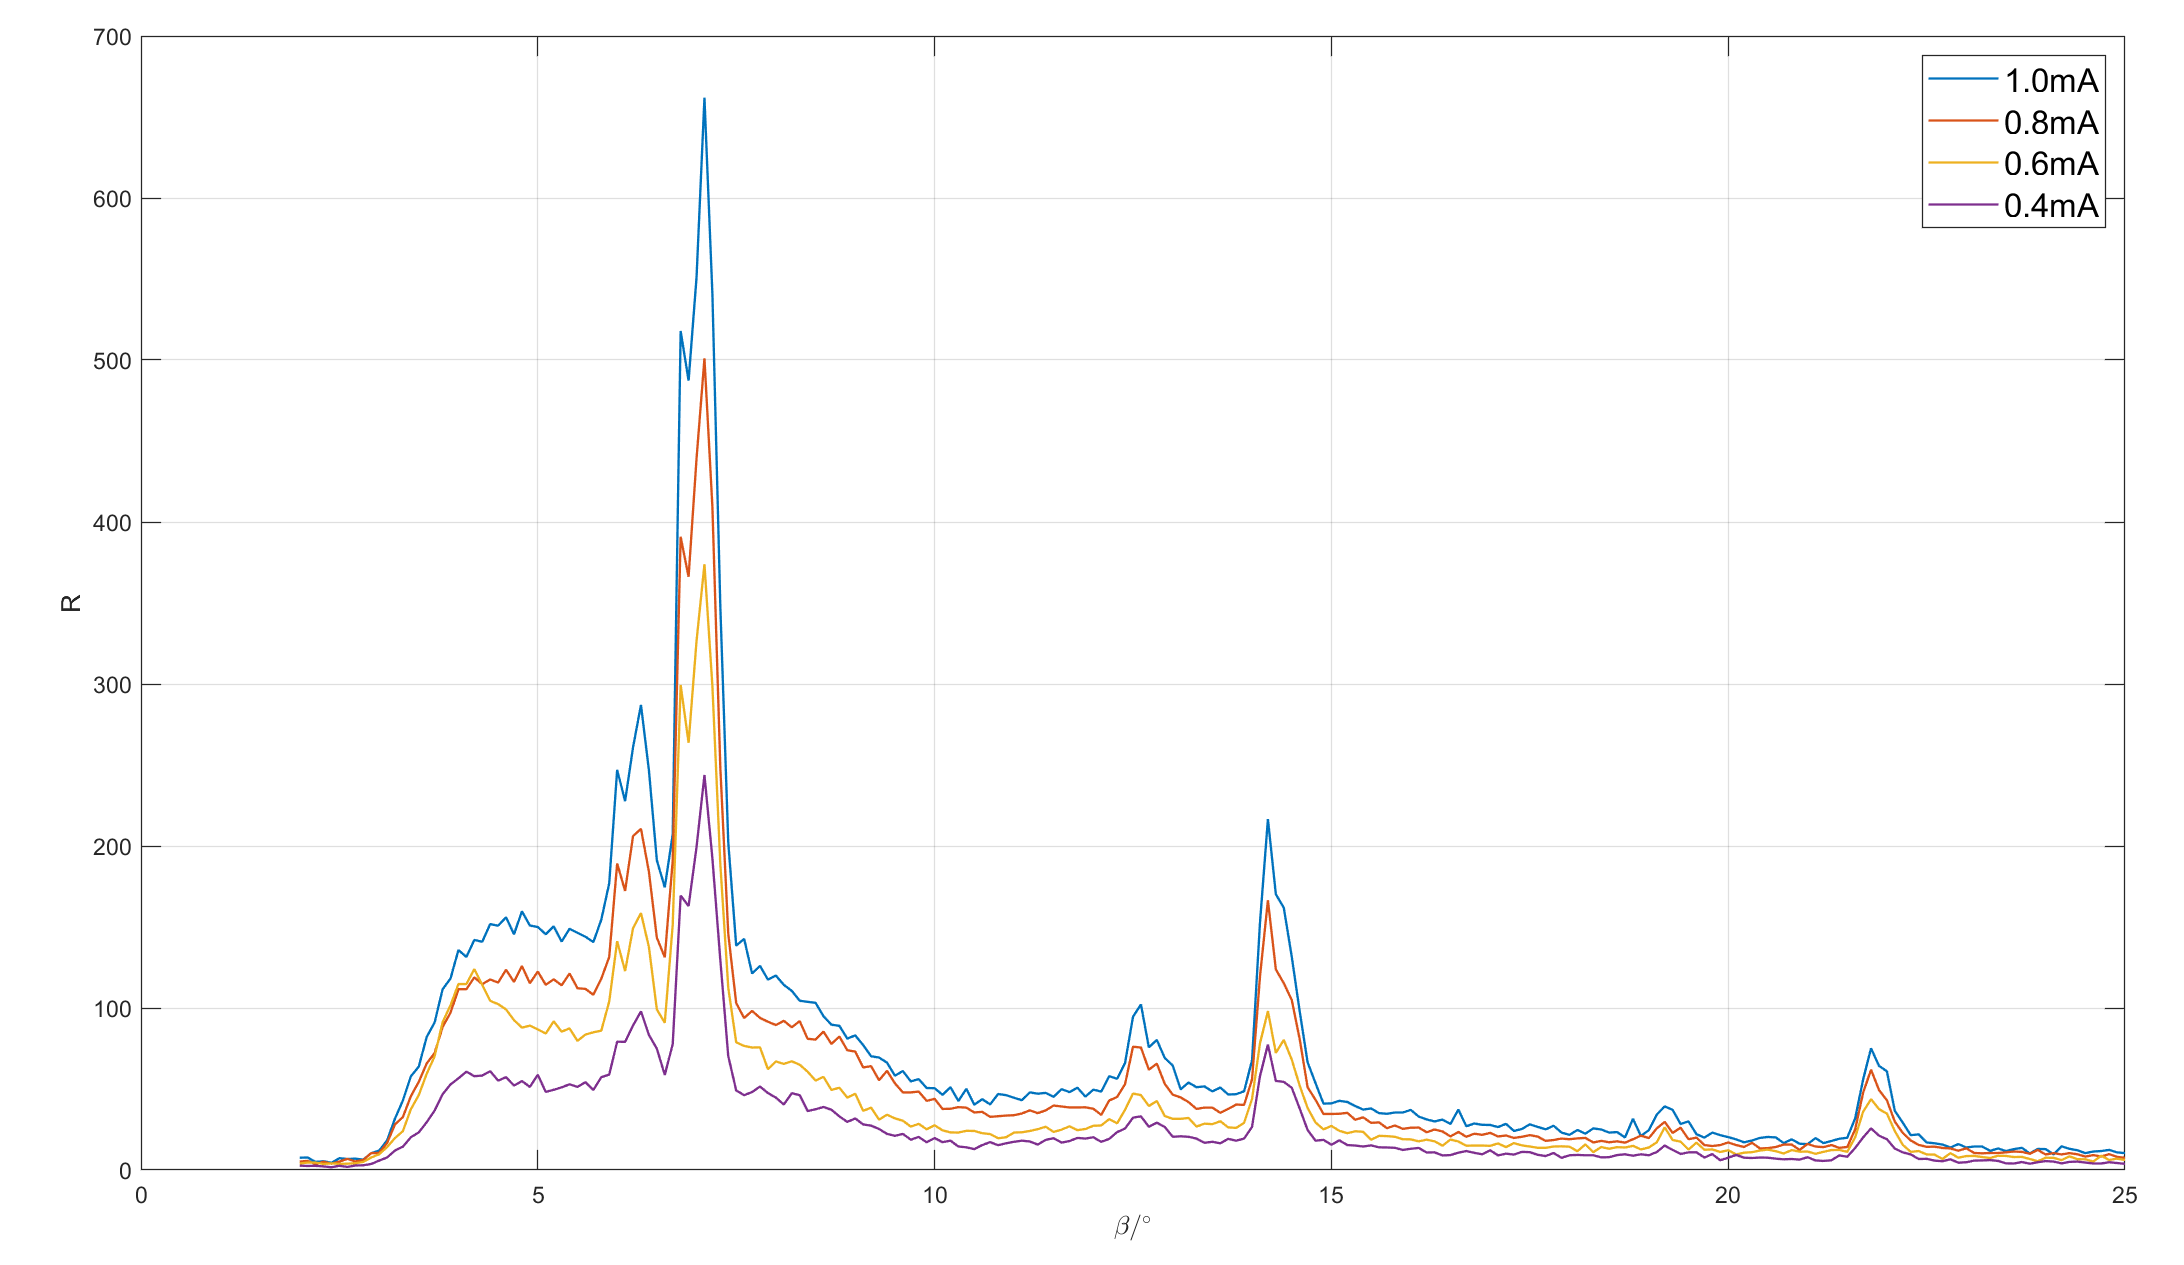
\includegraphics[scale=0.55]{current.png}
		\captionsetup{font=footnotesize}
		\caption{从上到下电流为$1,0.8,0.6,0.4$ mA对应相对强度随样平台转过角度$\beta$的变化情况}
	\end{figure}
	从Figure 7我们可以观察到
	\begin{itemize}
		\item 管电压$U=35 $kV不变,增大管电流$I$,各种波长X射线相对强度增加
		\item 针对标识谱,可以看到改变电流时,峰值波长对应的样平台转过角度$\beta$不变,即峰值波长$\lambda$不变,故X 射线标识谱峰位与管电流无关。
	\end{itemize}
	\section{总结}
	本实验使用X射线衍射仪研究了单晶的布拉格衍射,研究发现钼靶材料对应的X射线标识谱只有两条峰值波长,分别为:$\lambda_1=0.061$ nm,$\lambda_2=0.069$ nm;接下来,我们研究了X 射线管的电压对于它发出的X射线谱的影响,发现针对连续谱,随着管电压V升高,所有波长的X射线强度均增加,同时短波限$\lambda_{\min}$向短波方向移动,针对标识谱,X射线标识谱峰位与管电压无关;随后,我们通过研究发现钼靶临界值$V_{\text{th}}$,并根据不同电压对应的短波极限波长不同,验证了Duane-Hunt关系,并根据所得数据计算出普朗克常量$h=6.7119\times10^{-34}\;\text{J}\cdot\text{s}$,相对误差为1.29\%;最后,我们研究了X射线管的电流对于它发出的X射线谱的影响,发现增大管电流$I$,各种波长X射线相对强度增加,针对标识谱,X射线标识谱峰位与管电流无关。
	\appendix
	%\section{附录:原始数据}
	%\begin{figure}[H]
	%	\centering
	%	\includegraphics[scale=0.25]{originaldata.jpg}
	%\end{figure}
	\phantomsection
	\addcontentsline{toc}{section}{参考文献}
	\bibliographystyle{plain}
	\bibliography{Gal}
\end{document}